% Generated from the public primitive catalog. Original Atlas drawing; Apache-2.0.
% Target: present; view: overview
\documentclass[border=9pt]{standalone}
% Original Atlas figure theme. Apache-2.0; see the repository LICENSE.
\usepackage[T1]{fontenc}
\usepackage{lmodern}
\usepackage{amsmath,amssymb}
\usepackage{tikz}
\usetikzlibrary{arrows.meta,positioning,calc,fit,backgrounds,decorations.pathreplacing,matrix}
\definecolor{atlasInk}{HTML}{172235}
\definecolor{atlasTeal}{HTML}{0D7B7D}
\definecolor{atlasMuted}{HTML}{637278}
\definecolor{atlasFill}{HTML}{EAF4F2}
\definecolor{atlasLine}{HTML}{B6C8C7}
\tikzset{
  every picture/.style={line width=.65pt,draw=atlasInk,>=Latex},
  every node/.style={text=atlasInk,font=\sffamily\small},
  box/.style={draw,rounded corners=1.5pt,minimum height=.9cm,minimum width=1.6cm,align=center,inner sep=6pt,fill=white},
  accent/.style={box,draw=atlasTeal,fill=atlasFill},
  wire/.style={->,line width=.7pt},
  keywire/.style={wire,draw=atlasTeal,dashed},
  xor/.style={draw,circle,fill=white,inner sep=0pt,minimum size=.38cm},
  add/.style={draw,rectangle,fill=white,inner sep=0pt,minimum size=.38cm},
  note/.style={font=\sffamily\scriptsize,text=atlasMuted,align=center},
  phase/.style={font=\sffamily\small\bfseries,text=atlasTeal},
  group/.style={draw=atlasLine,dashed,rounded corners=2pt,inner sep=8pt}
}
\newcommand{\rotl}{\mathbin{\lll}}
\newcommand{\rotr}{\mathbin{\ggg}}
\newcommand{\kx}{\operatorname{Keccak}\!\text{-}\!f[1600]}

\newcommand{\AtlasKeyBits}{k}
\newcommand{\AtlasKeyWords}{N_k}
\newcommand{\AtlasRounds}{31}
\newcommand{\AtlasPriorRounds}{30}
\newcommand{\AtlasRoundKeys}{32}
\newcommand{\AtlasDoubleRounds}{15.5}
\newcommand{\AtlasSixRoundGroups}{5.166666666666667}
\newcommand{\AtlasFLGroups}{4.166666666666667}
\newcommand{\AtlasRoundStart}{-7}
\newcommand{\AtlasBlockBits}{64}
\newcommand{\AtlasOutputBits}{d}
\newcommand{\AtlasStateBits}{8w}
\newcommand{\AtlasNonceBits}{v}
\newcommand{\AtlasCounterBits}{q}
\newcommand{\AtlasStreamBlockBits}{b}
\newcommand{\AtlasRate}{r}
\newcommand{\AtlasCapacity}{c}
\newcommand{\AtlasSteps}{N}
\newcommand{\AtlasLastStep}{N-1}
\newcommand{\AtlasWordBits}{w}
\newcommand{\AtlasHashWords}{h}
\newcommand{\AtlasFeedForward}{\boxplus}
\newcommand{\AtlasByteOrder}{big-endian}
\newcommand{\AtlasDomain}{01}
\newif\ifAtlasXof
\AtlasXoffalse
\begin{document}
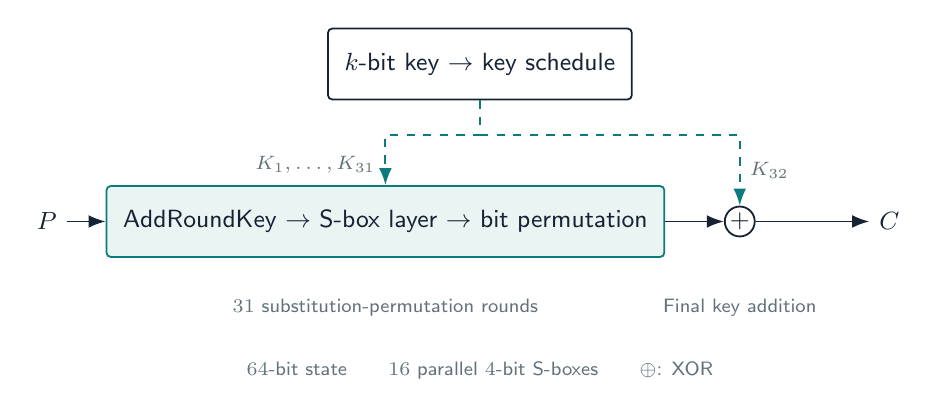
\begin{tikzpicture}
  \node (in) at (0,0) {$P$};
  \node[accent,minimum width=6cm] (rounds) at (4.3,0) {AddRoundKey $\to$ S-box layer $\to$ bit permutation};
  \node[xor] (last) at (8.8,0) {$+$};
  \node (out) at (10.7,0) {$C$};
  \draw[wire] (in) -- (rounds); \draw[wire] (rounds) -- (last); \draw[wire] (last) -- (out);
  \node[box] (schedule) at (5.5,2) {$\AtlasKeyBits$-bit key $\to$ key schedule};
  \draw[keywire] (schedule.south) -- (5.5,1.1) -| node[left,note,pos=.8] {$K_1,\ldots,K_{\AtlasRounds}$} (rounds.north);
  \draw[keywire] (5.5,1.1) -- (8.8,1.1) -- node[right,note] {$K_{\AtlasRoundKeys}$} (last.north);
  \node[note] at (4.3,-1.1) {$\AtlasRounds$ substitution-permutation rounds};
  \node[note] at (8.8,-1.1) {Final key addition};
  \node[note] at (5.5,-1.9) {$\AtlasBlockBits$-bit state\qquad $16$ parallel $4$-bit S-boxes\qquad $\oplus$: XOR};
\end{tikzpicture}

\end{document}
